%Este trabalho está licenciado sob a Licença Creative Commons Atribuição-CompartilhaIgual 4.0 Internacional. Para ver uma cópia desta licença, visite https://creativecommons.org/licenses/by-sa/4.0/ ou envie uma carta para Creative Commons, PO Box 1866, Mountain View, CA 94042, USA.

\chapter{Expressões algébricas}

\begin{obs}
  Expressões algébricas são expressões matemáticas que envolvem números, letras e operações.
\end{obs}

 Por exemplo:
 \begin{gather*}
  2x,\\
  x^2+1,\\
  x(x+3),\\
  2x+3y,\\
  %x^2 + 2y + 3z -4= 52, \\
  \dfrac{14x + 8y}{2x}, \\
  \dfrac{2}{5}x^3 + 3\sqrt{x^4}.
  %5x(x+3)-4x(2-x)=7.
 \end{gather*}

 Nestas expressões as letras que aparecem são chamadas de \textbf{variáveis}, e os números que aparecem multiplicando uma letra são chamados de \textbf{coeficientes}.

 As expressões algébricas são utilizadas dentre outras coisas, para descrever uma situação problema na qual não conhecemos todos os valores envolvidos, representar uma fórmula, ou expressar uma equação. Devido a sua importância, precisamos compreender como se comportam as operações presentes nas expressões algébricas. Em outras palavras, ``como fazer contas com letras''.

\section{Operações algébricas}


\subsection{Adição e subtração}

 Podemos somar somente letras iguais e com mesmo expoente. Por exemplo:

 \begin{itemize}
  \item $2x + x= (2+1)x= 3x$;
  \item $x^2 - 3x^2= (1-3)x^2= -2x^2$;
  \item $2x + y + 5x^2 + 7y - 3x= 5x^2 + (2-3)x + (1+7)y= 5x^2 - 1x + 8y$;
  \item $3(x+ 4y-2)= 3x + 3.4y - 3.2= 3x + 12y - 6$;
  \item $\dfrac{3x^2}{4}+\dfrac{x}{2}= \dfrac{3x^2 + 2x}{4}$.
 \end{itemize}

 \subsection{Multiplicação}

 Na multiplicação devemos sempre multiplicar coeficiente por coeficiente e letra por letra. Sendo que no caso das letras serem iguais, devemos manter a letra e somar seus expoentes, e no caso das letras serem diferentes apenas fazemos a associação das duas letras. Por exemplo:

  \begin{itemize}
   \item $x \cdot x = x^{1+1}= x^2$;
   \item $x \cdot x^2= x^{1+2}= x^3$;
   \item $x \cdot 2y= (1 \cdot 2)xy= 2xy$;
   \item $3x \cdot 2x^2y= (3 \cdot 2)x^{1+2}y= 6x^3y$;
   \item $4x^4 \cdot \dfrac{1}{2x^{2}}= 4x^4 \cdot \dfrac{1}{2}x^{-2}= (4 \cdot \dfrac{1}{2})x^{4-2}= 2x^2$;
   \item $(x - 1) \cdot (x - 2)= x(x-2) - 1(x-2)= x^2 -2x -x +2= x^2 - 3x + 2$.
  \end{itemize}

   \subsection{Divisão}

   Na divisão podemos simplificar fatores em comum do numerador e denominador. Quando temos letras iguais, devemos manter a letra e subtrair seus expoentes, e no caso das letras serem diferentes apenas fazemos a associação das duas letras. Por exemplo:

  \begin{itemize}
   \item $x \div x= x^{1-1}= x^0= 1$;
   \item $x \div x^2= x^{1-2}= x^{-1}= \dfrac{1}{x}$;
   \item $2y \div x= \dfrac{2y}{x}$;
   \item $4y^3 \div 2y^2= \dfrac{4}{2} \cdot \dfrac{y^3}{y^2}= 2y^{3-2}= 2y$;
   \item $\dfrac{x^2yz^3}{x^2y^3z^2}= x^{2-2}y^{1-3}z^{3-2}= x^0 y^{-2}z^{1}= \dfrac{z}{y^2}$;
   \item $\dfrac{(x+3) \cdot (x-1)}{(x-1)\cdot (2x+3)}= \dfrac{x+3}{2x+3}$.
  \end{itemize}


  \subsection{Potenciação}

  Na potenciação devemos aplicar o expoente ao coeficiente e à incógnita, obedecendo as propriedades de potência. Por exemplo:

    \begin{itemize}
     \item $(2x)^2= 2^2 \cdot x^2= 4x^2$;
     \item $(3x^2)^3= 3^3 \cdot x^{2\cdot 3}= 27x^6$;
     \item $(x+1)^2= (x+1) \cdot (x+1)= x^2 + 2x +1$;
     \item $(x-1)^2= (x-1) \cdot (x-1)= x^2 - 2x +1$;
     \item $\left(\dfrac{3a^2}{4}\right)^2= \dfrac{3^2 a^{2 \cdot 2}}{4^2}= \dfrac{9a^4}{16}$.
    \end{itemize}


  \subsection{Radiciação}

  Na radiciação devemos extrair a raiz do coeficiente e da incógnita. Observamos que para uma radiciação cujo radicando é uma expressão algébrica devemos aplicar as propriedades de radiciação do capítulo anterior. Por exemplo:
    \begin{itemize}
     \item $\sqrt{x}= x^{\frac{1}{2}}$;
     %\item $\sqrt{x^2}= \abs{x}$;
     \item $\sqrt{x^4}= (x^4)^{\frac{1}{2}}= x^{\frac{4}{2}}= x^2$;
     \item $\sqrt[3]{8x^6}= \sqrt[3]{8} \cdot \sqrt[3]{x^6}=\sqrt[3]{2^3} \cdot \sqrt[3]{x^6} = 2^{\frac{3}{3}} x^{\frac{6}{3}}= 2x^2$;
     \item $\sqrt{\dfrac{2x^5}{16}}= \dfrac{\sqrt{2x^5}}{\sqrt{4^2}}= \dfrac{\sqrt{2} x^{\frac{5}{2}}}{4}= \dfrac{x^{2} \sqrt{2x}}{4}$.
     
    \end{itemize}


  \subsection{Fatoração das expressões algébricas}


 A fatoração das expressões algébricas, é o que nos permite escrever a expressão como um produto de dois termos. Ela é utilizada principalmente na resolução de equações, para acelerar o processo de resolução.

 Os seguintes casos de fatoração são os mais utilizados:
 \begin{itemize}
  \item Fator em comum: 
 \begin{gather*}
   x^2 + x= x(x + 1) \\
   4x^2 + 6= 2(2x^2 + 3)
 \end{gather*}
  
  \item Agrupamento:
 \begin{equation*}
   ax + bx + ay + by= (a+b)x+(a+b)y= (a+b)(x+y)
 \end{equation*}
\end{itemize}
  
 \section{Produtos notáveis}

 \begin{itemize}
  \item Trinômio do quadrado perfeito ($+$): 
\begin{eqnarray*}
(x + y)^2&=& (x+y) \cdot (x+y)\\
         &=& x^2 + xy + yx + y^2 \\
         &=& x^2 + 2xy + y^2
\end{eqnarray*}

  \item Trinômio do quadrado perfeito ($-$): 
\begin{eqnarray*}
(x - y)^2&=& (x - y) \cdot (x - y) \\
         &=& x^2 - xy - yx + y^2 \\
         &=& x^2 - 2xy + y^2
\end{eqnarray*}

  \item Diferença de dois quadrados: 
\begin{equation*}
(x + y) \cdot (x - y)= x^2 - xy + yx - y^2 = x^2 - y^2
\end{equation*}

  \item Cubo perfeito ($+$): 
\begin{eqnarray*}
(x+y)^3&=& (x+y)^2 \cdot (x+y) \\
       &=& (x^2 + 2xy + y^2) \cdot (x+y) \\
       &=& x^3 + 3x^2y + 3xy^2 + y^3
\end{eqnarray*}

  \item Cubo perfeito ($-$): 
\begin{eqnarray*}
(x-y)^3&=& (x-y)^2 \cdot (x-y) \\
       &=& (x^2 - 2xy + y^2) \cdot (x-y) \\
       &=& x^3 - 3x^2y + 3xy^2 - y^3
\end{eqnarray*}

  \item Diferença de dois cubos:
\begin{equation*}
x^3 - y^3= (x-y) \cdot (x^2 + xy + y^2)
\end{equation*}

\item Diferença de potências do ordem $n$:
\begin{equation*}
x^n - y^n= (x-y) \cdot (x^{n-1} + x^{n-2}y + x^{n-3}y^2 + \cdots + xy^{n-2} + y^{n-1})
\end{equation*}
 \end{itemize}
 
%  \section{Binômio de Newton}
 
%  As expressões $(x + y)^2$ e $(x + y)^3$ para $x, y \in \R$,podem ser generalizadas para $(x + y)^n$ com $n \in \N$, esta generalização é dada pelo Binômio de Newton, da seguinte forma:
 
% \begin{equation*}
% (x + y)^n= \sum^{n}_{k=0} \binom{n}{k} \cdot x^{n-k} y^{k}= \sum^{n}_{k=0} \binom{n}{k} \cdot x^{k} y^{n-k} 
% \end{equation*}
 
% \begin{eqnarray}
% (x - y)^n &=& (x +(-y))^n= \sum^{n}_{k=0} \binom{n}{k} \cdot x^{n-k} (-y)^{k} \\
%           &=& \sum^{n}_{k=0} \binom{n}{k} \cdot x^{n-k} (-1)^{k}y^{k} \\
%           &=& \sum^{n}_{k=0} (-1)^{k} \binom{n}{k} \cdot x^{n-k} y^{k}
% \end{eqnarray}
 
%  Os coeficientes $\binom{n}{k}$ são chamados coeficientes binomiais e são definidos por:
 
% \begin{equation*}
% \binom{n}{k}= \frac{n!}{k!(n-k)!}
% \end{equation*}

%  para $n, k \in \N$ com $k \leq n$. 
 
%  Vale lembrar que por definição o fatorial de $n$ é dado por:
% \begin{equation*}
% n!= n \cdot (n-1) \cdot (n-2) \cdots 2 \cdot 1 \ .
% \end{equation*}


 
\section{Completamento de Quadrados}

O processo de completar quadrados tem base nas fórmulas de produtos notáveis $(x+y)^2$ e $(x-y)^2$, fazendo-se uma comparação direta entre os termos.
\begin{exem}
  Completar quadrados de $x^2+6x$. Temos que descobrir $y$ de forma que $x^2+6x$ possa ser comparado com $(x+y)^2=x^2+2xy+y^2$. Veja que tomando $2xy=6x$, ou seja, $y=3$, temos que
  \begin{equation*}
      x^2+6x = (x+3)^2-9.
  \end{equation*}
\end{exem}

\begin{exem}
  Completar quadrados de $x^2-x+2$.  Primeiramente, vamos desconsiderar a constante. Vamos comparar $x^2-x$ com $(x-y)^2=x^2+2xy+y^2$. Veja que tomando $2xy=x$, ou seja, $y=\frac{1}{2}$, temos que
  $$x^2-x+2 = \left(x-\frac{1}{2}\right)^2-\frac{1}{4}+2 = \left(x-\frac{1}{2}\right)^2+\frac{7}{4}.$$
\end{exem}

O termo ``completamento de quadrados'' tem uma motivação geométrica. Por exemplo, para completar quadrado da expressão $x^2+6x$ podemos pensar na construção geométrica
\begin{center}
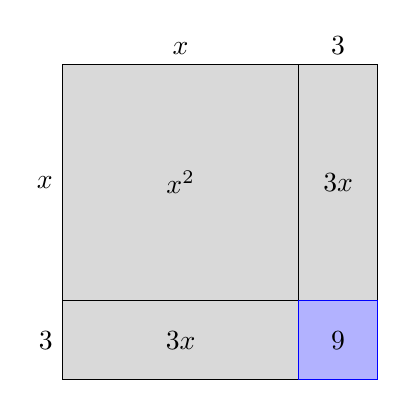
\begin{tikzpicture}[y=-1cm]
    \fill[gray!30,draw=black] (0,0) rectangle (3,3);
    \fill[gray!30,draw=black] (0,3) rectangle (3,4);
    \fill[gray!30,draw=black] (3,0) rectangle (4,3);
    \fill[blue!30,draw=blue] (3,3) rectangle (4,4);
    \draw (1.5,0) node[above]{$x$};
    \draw (0,1.5) node[left]{$x$};
    \draw (3.5,0) node[above]{$3$};
    \draw (0,3.5) node[left]{$3$};
    \draw (1.5,1.5) node{$x^2$};
    \draw (1.5,3.5) node{$3x$};
    \draw (3.5,1.5) node{$3x$};
    \draw (3.5,3.5) node{$9$};
\end{tikzpicture}
\end{center}

Assim, vemos que $x^2+6x$ corresponde à área da região cinza. Para completar a área de todo quadrado de lado $x+3$, faltaria considerar a área do quadrado azul.

\section{Expressões algébricas racionais}
 
 Vejamos alguns exemplos expressões algébricas racionais:
 \begin{exem}    
  $\dfrac{6x^7 x^6}{3x^3x^8}$
\begin{equation*}
\dfrac{6x^7 x^6}{3x^3x^8}= \dfrac{6x^{7+6}}{3x^{3+8}}= \dfrac{6x^{13}}{3x^{11}}= 2x^{13-11}= 2x^2 \ ;
\end{equation*}
 \end{exem}
 
 \begin{exem}
  $\dfrac{4x^0y^5z^3}{12z^3y^4x^3}$
\begin{equation*}
\dfrac{4x^0y^5z^3}{12z^3y^4x^3}= \dfrac{4x^0y^5z^3}{12x^3y^4z^3}= \dfrac{4}{12} \cdot \dfrac{x^0}{x^3} \cdot \dfrac{y^5}{y^4} \cdot \dfrac{z^3}{z^3}= \dfrac{1}{4} \cdot \dfrac{1}{x^3} \cdot y \cdot 1=\dfrac{y}{3x^3} \ ;
\end{equation*}
  \end{exem}
 
 \begin{exem}
  $\dfrac{x^2+2x^5}{x^3}= \dfrac{x^2(1+2x^3)}{x^2 x}= \dfrac{1+2x^3}{x}$;
 \end{exem}
 
 \begin{exem}
  $\left(\dfrac{4x^3y^2}{3z^3}\right) \cdot \left(\dfrac{z}{2x^2y} \right)^3$
\begin{equation*}
\left(\dfrac{4x^3y^2}{3z^3}\right) \cdot \left(\dfrac{z}{2x^2y} \right)^3 = \left(\dfrac{4x^3y^2}{3z^3}\right) \cdot \left(\dfrac{z^3}{2^3(x^2)^3y^3} \right)= \dfrac{4x^3y^2z^3}{3z^38x^6y^3}= \dfrac{1}{6x^3y} \ ;
\end{equation*}
  \end{exem}
 
 \begin{exem}
 $\dfrac{x^2 - 4}{x^4 - 2x^3}$
\begin{equation*}
\dfrac{x^2 - 4}{x^4 - 2x^3}= \dfrac{(x+2) \cdot (x-2)}{x^3 \cdot (x - 2)}= \dfrac{x+2}{x^3} \ ; 
\end{equation*}
  \end{exem}

  \begin{exem}
  $\dfrac{2xy-1}{x^2 - y^2} + \dfrac{4x}{x-y}$
  \begin{eqnarray*}
   \dfrac{2xy-1}{x^2 - y^2} + \dfrac{4x}{x-y} &=& \dfrac{2xy-1}{(x-y)\cdot (x+y)} + \dfrac{4x}{x-y} \\
   &=& \dfrac{2xy-1}{(x-y)\cdot (x+y)} + \dfrac{4x \cdot (x+y)}{(x-y)\cdot (x+y)} \\
   &=& \dfrac{2xy - 1 + 4x^2 + 4xy}{(x-y)\cdot (x+y)} \\
   &=& \dfrac{6xy - 1 + 4x^2}{x^2 - y^2} \ ;
  \end{eqnarray*}
  \end{exem}
  
 \begin{exem}
  $\dfrac{2y}{z} \cdot \left( \dfrac{z}{x^3} - \dfrac{3z}{x^4y^4} \right) + \left( \dfrac{zy}{x^2} \right)^{-2}$
  
  \begin{eqnarray*}
   \dfrac{2y}{z} \cdot \left( \dfrac{z}{x^3} - \dfrac{3z}{x^4y^4} \right) + \left( \dfrac{zy}{x^2} \right)^{-2} 
   &=& \dfrac{2y}{z} \cdot \left( \dfrac{zxy^4}{x^4y^4} - \dfrac{3z}{x^4y^4} \right) + \left( \dfrac{x^2}{zy} \right)^{2} \\
   &=& \dfrac{2y}{z} \cdot \left( \dfrac{zxy^4 - 3z}{x^4y^4} \right) + \left( \dfrac{x^4}{z^2y^2} \right) \\
   &=& \left( \dfrac{2zxy^5 - 6yz}{x^4y^4z} \right) + \left( \dfrac{x^4}{z^2y^2} \right) \\
   &=& \left( \dfrac{yz(2xy^4 - 6)}{x^4y^4z} \right) + \left( \dfrac{x^4}{z^2y^2} \right) \\
   &=& \left( \dfrac{2xy^4 - 6}{x^4y^3} \right) + \left( \dfrac{x^4}{z^2y^2} \right) \\
   &=& \left( \dfrac{(2xy^4 - 6) \cdot (z^2)}{x^4y^3z^2} \right) + \left( \dfrac{x^4 \cdot (x^4y)}{x^4y^3z^2} \right) \\
   &=& \left( \dfrac{2xy^4z^2 - 6z^2}{x^4y^3z^2} \right) + \left( \dfrac{x^8y}{x^4y^3z^2} \right) \\
   &=& \dfrac{2xy^4z^2 - 6z^2 + x^8y}{x^4y^3z^2} \ ;
  \end{eqnarray*}
 \end{exem}

 
 % \begin{exem}
 %  $\dfrac{-4x^2}{x^3 - y^3} + \dfrac{4}{x-y}$
 %  \begin{eqnarray*}
 %   \dfrac{-4x^2}{x^3 - y^3} + \dfrac{4}{x-y} & = & \dfrac{-4x^2}{(x-y)\cdot (x^2+xy+y^2)} + \dfrac{4}{x-y} \\
 %   &=& \dfrac{-4x^2}{(x-y)\cdot (x^2+xy+y^2)} + \dfrac{4 \cdot (x^2+xy+y^2)}{(x-y)\cdot (x^2+xy+y^2)} \\
 %   &=& \dfrac{-4x^2 + 4x^2 + 4xy + 4y^2}{(x-y) \cdot (x^2+xy+y^2)} \\
 %   &=& \dfrac{4xy + 4y^2}{x^3 - y^3}  \ ;
 %  \end{eqnarray*}
 %  \end{exem}

 \section{Expressões algébricas radicais ou irracionais}
 
 Vejamos alguns exemplos de expressões algébricas radicais;
 
 \begin{exem}   
   $x^{\frac{5}{7}} \cdot x^{\frac{10}{7}} \cdot x^{\frac{6}{7}}$
\begin{equation*}
x^{\frac{5}{7}} \cdot x^{\frac{10}{7}} \cdot x^{\frac{6}{7}}= x^{\frac{5+10+6}{7}}= x^{\frac{21}{7}}= x^3 \ ;
\end{equation*}
    \end{exem}
 
 \begin{exem}
   $\dfrac{\sqrt[5]{x^2}}{x} \cdot \dfrac{\sqrt[5]{x^3}}{y^2} \cdot y^{\frac{3}{2}}$
\begin{equation*}
\dfrac{\sqrt[5]{x^2}}{x} \cdot \dfrac{\sqrt[5]{x^3}}{y^2} \cdot y^{\frac{3}{2}}= \dfrac{\sqrt[5]{x^{2+3}}}{x} \cdot y^{\frac{3}{2} - 2}= \dfrac{x}{x} \cdot y^{\frac{-1}{2}}= \dfrac{1}{\sqrt{y}}= \dfrac{1}{\sqrt{y}} \cdot \dfrac{\sqrt{y}}{\sqrt{y}}= \dfrac{\sqrt{y}}{y} \ ;
\end{equation*}
   \end{exem}
 
 \begin{exem}
    $\sqrt{x^5} \cdot \sqrt[3]{x}$
\begin{equation*}
\sqrt{x^5} \cdot \sqrt[3]{x}= x^{\frac{5}{2}} \cdot x^{\frac{1}{3}}= x^{\frac{15+2}{6}} = x^{\frac{17}{6}} = \sqrt[6]{x^{6+6+5}}= \sqrt[6]{x^6 x^6 x^5} =  x^2 \cdot \sqrt[6]{x^5} \ ;
\end{equation*}
   \end{exem}
 
 \begin{exem}
   $\sqrt{\sqrt[3]{x^{10}}}$
\begin{equation*}
\sqrt{\sqrt[3]{x^{10}}}= (x^{\frac{10}{3}})^{\frac{1}{2}}= x^{\frac{5}{3}}= \sqrt[3]{x^5}= \sqrt[3]{x^3 \cdot x^2}= x \sqrt[3]{x^2} \ ;
\end{equation*}
   \end{exem}
 
 \begin{exem}
    $(\sqrt{x} + 2) \cdot (\sqrt{x} - 2)$
\begin{equation*}
(\sqrt{x} + 2) \cdot (\sqrt{x} - 2)= (\sqrt{x})^2 - 4= x-4 \ ;
\end{equation*}
   \end{exem}
 
 \begin{exem}
  $(\sqrt[3]{x} - 2) \cdot (\sqrt[3]{x^2} + 2 \sqrt[3]{x} + 4)$
\begin{equation*}
(\sqrt[3]{x} - 2) \cdot (\sqrt[3]{x^2} + 2 \sqrt[3]{x} + 4)= \sqrt[3]{x^3} + 2\sqrt[3]{x^2} + 4 \sqrt[3]{x} - 2\sqrt[3]{x^2}- 4 \sqrt[3]{x} - 8= x - 8 \ ;
\end{equation*}
   \end{exem}
 
 \begin{exem}
  $\dfrac{125^{\frac{1}{3}}}{\sqrt{2x}} \cdot \sqrt{\dfrac{x}{98}}$
\begin{equation*}
\dfrac{125^{\frac{1}{3}}}{\sqrt{2x}} \cdot \sqrt{\dfrac{x}{98}}= \sqrt[3]{125} \cdot \sqrt{\dfrac{x}{98 \cdot 2x}}= \sqrt[3]{5^3} \cdot \sqrt{\dfrac{x}{196x}}= 5 \cdot \dfrac{1}{\sqrt{196}}= \dfrac{5}{14} \ ;
\end{equation*}
   \end{exem}
 
 \begin{exem}
   $\dfrac{3\sqrt{x}}{x-4} - \dfrac{\sqrt{x}}{\sqrt{x}+2}$
   \begin{eqnarray*}
    \dfrac{3\sqrt{x}}{x-4} - \dfrac{\sqrt{x}}{\sqrt{x}+2} &=& \dfrac{3\sqrt{x}}{(\sqrt{x}+2) \cdot (\sqrt{x}-2)} - \dfrac{\sqrt{x}}{\sqrt{x}+2} \\
    &=& \dfrac{3\sqrt{x}}{(\sqrt{x}+2) \cdot (\sqrt{x}-2)} - \dfrac{\sqrt{x} \cdot (\sqrt{x}-2)}{(\sqrt{x}+2) \cdot (\sqrt{x}-2)} \\
    &=& \dfrac{3\sqrt{x} - x + 2\sqrt{x}}{(\sqrt{x}+2) \cdot (\sqrt{x}-2)} \\
    &=& \dfrac{5\sqrt{x} - x}{x-4}
   \end{eqnarray*}
 \end{exem}
 
\newpage
\begin{secExercicios}

\begin{exer}
    Fatorar:
    \begin{multicols}{2}
        \begin{enumerate}[a)]
            \item $6x+x^2$
            \item $x^2-25$
            \item $16x^2-a^4$
            \item $y^7-1$
            \item $x^6+2x^4+x^2$
            \item $x^5-6x^3+9x$
        \end{enumerate}
    \end{multicols}
\end{exer}

\begin{exer}
  Complete os quadrados:
  \begin{enumerate}[a)]\begin{multicols}{2}
    \item $x^2-4x$
    \item $-x^2+8x+3$
    \item $x^4-2x^2+2$
    \item $x^2+2x+7$
    \item $x-9x^2$
    \item $x^4-3x^2+1$
    \end{multicols}\end{enumerate}
\end{exer}

\begin{exer}
Aplicando o conceito de produtos notáveis, qual expressão algébrica obtemos após simplificar corretamente a seguinte expressão?
\[\dfrac{(2m+3)^2-2(2m+3)(m-2)+(m-2)^2}{(m+5)(m-5)}\]
\end{exer}
\begin{resp}
 $\dfrac{m+5}{m-5}$
\end{resp}

\begin{exer}
Aplicando o conceito de produtos notáveis, qual expressão algébrica obtemos após simplificar corretamente a seguinte divisão de frações algébricas?
\[\dfrac{\dfrac{3}{x+1}}{\dfrac{3x+6}{x^2-1}}\]
\end{exer}
\begin{resp}
 $\dfrac{x-1}{x+2}$
\end{resp}

\begin{exer}
  Simplificando a expressão $(x + 5)^2 - x(x + 10)$, encontraremos:
  \begin{enumerate}[a)]\begin{multicols}{5}
  \item 25
  \item 30
  \item 50
  \item 75
  \item 100
  \end{multicols}\end{enumerate}
\end{exer}
\begin{exer}
  Resolva os produtos notáveis da expressão $(2x - 5) (2x + 5) - (2x - 5)^2$.
\end{exer}

\begin{exer}
  Simplifique as expressões abaixo:
  \begin{enumerate}[a)]\begin{multicols}{2}
  
        \item $\dfrac{4a^2 b^3-6b^2a^3}{2a^2b}$
        
        \item $\dfrac{x^2 +x - 6}{x-2}$
  
        \item $\dfrac{x^2 -4x}{x^2 - 3x - 4}$
        
       \item $\dfrac{x^2 + 5x +4}{x^2 + 3x - 4}$
  
       \item $\dfrac{x^3-1}{x^2 -1}$
  
        \item $\dfrac{x^4 - 16}{x-2}$

        \item $\dfrac{(3 + h)^2 - 9}{h}$
        
        \item $\dfrac{t^2 - 9}{2t^2 + 7t +3}$
        
        \item $\dfrac{(1+h)^4 - 1}{h}$
        
        \item $\dfrac{(2+h)^3 - 8}{h}$
  
        \item $\dfrac{\frac{1}{4} + \frac{1}{x}}{4+x}$
  
        \item $\dfrac{1}{t} - \dfrac{1}{t^2 + t}$

        \item $\dfrac{x^2 -4x}{x^2 - 3x - 4}$
  
        \item $\dfrac{(3 + h)^{-1} - 3^{-1}}{h}$
  
        \item $\dfrac{x^3}{2x^2 - x}$
  
        \item $\dfrac{\dfrac{1}{x} - 1}{x-1}$
  
        \item $\dfrac{x^3 + 1}{x^2 - 1}$
  
        \item $\dfrac{\dfrac{1}{x-1} + \dfrac{1}{x+1}}{x}$
  
        \item $\dfrac{x^3 - 8}{x^4 - 16}$
        \item $\dfrac{(2+h)^2 - 16}{h}$
        \item $\dfrac{t^3 + 4t^2 + 4t}{(t+2)(t-3)}$
  \end{multicols}\end{enumerate}  
\end{exer}

\begin{exer}
  Encontre a diferença entre os números $1522^2$ e $1520^2$.  
\end{exer}

\begin{exer}  
  (Cefet/MG - 2017) Se $x$ e $y$ são dois números reais positivos, então podemos dizer que a expressão $M = \left(x\sqrt{\dfrac{y}{x}} + y\sqrt{\dfrac{x}{y}}\right)^2$ é igual a:
  \begin{enumerate}[a)]\begin{multicols}{4}
  \item $\sqrt{xy}$
  \item $2xy$
  \item $4xy$
  \item $2\sqrt{xy}$
  \end{multicols}\end{enumerate}
\end{exer}
\begin{exer}
  (UFRGS 2016) Se $x + y = 13$ e $x. y = 1$, então, $x^2 + y^2$ é:
  \begin{enumerate}[a)]\begin{multicols}{5}
  \item 166
  \item 167
  \item 168
  \item 169
  \item 170
  \end{multicols} \end{enumerate}
\end{exer}

\begin{exer}
  Realizando a simplificação da expressão algébrica $\dfrac{(2x+10)(2x-10)}{x^2 - 25},$ encontraremos:
  \begin{multicols}{5}
  \begin{enumerate}[a)]
        \item 1
        
         \item 2
        
        \item 3
        
       \item 4
        
        \item 5
    \end{enumerate}
  \end{multicols}
  
\end{exer}

\begin{exer}
  Qual é a forma fatorada do produto entre os polinômios $x^2 + 14x + 49$ e $x^2 - 14x + 49$?
  \begin{multicols}{2}
  \begin{enumerate}[a)]
        \item $(x + 7)^2(x - 7)^2$
        
       \item $(x + 7)(x - 7)^2$
        
       \item $(x + 7)^2x - 72$
        
        \item $x + 72(x - 7)^2$
        
        %\item $(x^2 + 14x + 49)(x^2 - 14x + 49)$
  \end{enumerate}
  \end{multicols}
  
\end{exer}

\begin{exer}
   A razão entre as formas fatoradas dos polinômios $ax + 2a + 5x + 10$ e $a^2 + 10a + 25$ é:
  \begin{enumerate}[a)]\begin{multicols}{2}
        \item $\dfrac{(a+5)(x-2)}{(a + 5)(a+5)}$
        
         \item $a+5$
        
        \item $a-5$
        
       \item $\dfrac{(x -2)}{a+5}$
        
        \item $\dfrac{x+2}{a+5}$
  \end{multicols}\end{enumerate}
\end{exer}

\begin{exer}
  Dado que $x$ e $y$ são valores reais onde $x \neq y$ e $x \neq -y$, o valor da expressão $$\left(\dfrac{x^{-2} - y^{-2}}{x^{-1}+y^{-1}}\right)\cdot\left(\dfrac{x^2 y+xy^2}{x^2 - y^2}\right)$$ é:
  \begin{enumerate}[a)]\begin{multicols}{5}
        \item -1
        
         \item -2
        
        \item 1
        
       \item 2
        
        \item 1/2
  \end{multicols}\end{enumerate}
  
\end{exer}

\begin{exer}
  Racionalize (numerador, denominador ou ambos):
  
  \begin{enumerate}[a)]\begin{multicols}{2}
        \item $\dfrac{\sqrt{t^2 + 9}-3}{t^2}$
        
         \item $\dfrac{\sqrt{x +2}-3}{x-7}$
        
        \item $\dfrac{x^2 - 81}{\sqrt{x} - 3}$
        
        \item $\dfrac{\sqrt{x}-x^2 }{1 - \sqrt{x}}$
  
        \item $\dfrac{\sqrt{x}-1 }{\sqrt{2x+3} - \sqrt{5}}$
  
        \item $\dfrac{\sqrt{1+h}-1 }{h}$
       
        \item $\dfrac{\sqrt{x^2 + 100} -10}{x^2}$
        
        \item $\dfrac{1}{t \sqrt{1 + t}} - \dfrac{1}{t}$
        
        \item $\dfrac{\sqrt[3]{x+2} -1}{x+1}$
  
        \item $\dfrac{\sqrt[4]{x} - \sqrt[4]{2}}{x-2}$
        
        \item $\dfrac{\sqrt[3]{x} - \sqrt[3]{3}}{x-3}$
  
        \item $\dfrac{\sqrt[3]{x}-1 }{\sqrt{x} - 1}$
  \end{multicols}\end{enumerate}
\end{exer}


% \begin{exer}
%   Qual é a forma simplificada da expressão algébrica $\dfrac{(x^2 + 14x + 49)(x^2 - 49)}{x^2 - 14x + 49}$?
  
%   \begin{enumerate}[a)]\begin{multicols}{3}
%         \item $\dfrac{(x + 7)(x+7)}{(x - 7)}$
        
%          \item $\dfrac{x + 7}{x - 7}$
        
%         \item $\dfrac{(x + 7)^3}{x - 7}$
        
%        \item $\dfrac{(x + 7)^2}{x - 7}$
        
%         \item $\dfrac{x^2 + 14x + 49}{x - 7}$
%   \end{multicols}\end{enumerate}
  
% \end{exer}

\begin{exer}
  A forma simplificada da razão entre as expressões $x^3 - 8y^3$ e $x^2 - 4xy + 4y^2$ é:
  \begin{enumerate}[a)]\begin{multicols}{2}
        \item $\dfrac{(x+4y)^2}{x-4y}$
        
         \item $\dfrac{x^2 + 2xy + 4y^2}{x-2y}$
        
        \item $\dfrac{(x+y)^2}{x-y}$
        
       \item $\dfrac{(2x+2)^2}{x-y}$
        
        \item $\dfrac{(x+y)^2}{2x-y}$
  \end{multicols}\end{enumerate}
\end{exer}

\begin{exer}
    Coloque na forma $(x-a)^2+(y-b)^2=r^2$.
    \begin{enumerate}[a)]
        \item $x^2+y^2-2x=0$
        \item $x^2+y^2-x-y=0$
        \item $x^2+y^2+3x-y=2$
    \end{enumerate}
    \end{exer}
% \begin{resp}
%     \par\noindent\rule{\columnwidth}{0.4pt}
% \end{resp}

% \begin{exer}
%   Simplifique as expressões abaixo:
  
%   \begin{enumerate}[a)]\begin{multicols}{3}
  
%         \item $\dfrac{x^2 -4x}{x^2 - 3x - 4}$
  
%         \item $\dfrac{(3 + h)^{-1} - 3^{-1}}{h}$
  
%         \item $\dfrac{x^3}{2x^2 - x}$
  
%         \item $\dfrac{\dfrac{1}{x} - 1}{x-1}$
  
%         \item $\dfrac{x^3 + 1}{x^2 - 1}$
  
%         \item $\dfrac{\dfrac{1}{x-1} + \dfrac{1}{x+1}}{x}$
  
%         \item $\dfrac{x^3 - 8}{x^4 - 16}$
%         \item $\dfrac{(2+h)^2 - 16}{h}$
%         \item $\dfrac{t^3 + 4t^2 + 4t}{(t+2)(t-3)}$
  
%   \end{multicols}\end{enumerate}
  
% \end{exer}
% \begin{exer}
%   Racionalize (numerador, denominador ou ambos):
  
%   \begin{enumerate}[a)]\begin{multicols}{3}
%         \item $\dfrac{9 - t}{3 - \sqrt{t}}$
        
%          \item $\dfrac{\sqrt{x}-1}{\sqrt[3]{x} - 1}$
        
%         \item $\dfrac{\sqrt[3]{x}-1}{\sqrt[4]{x} - 1}$
        
%        \item $\dfrac{3 - \sqrt{5+x}}{1 - \sqrt{5-x}}$
        
%         \item $\dfrac{\sqrt{1+x}-1 }{-x}$
  
%         \item $\dfrac{\sqrt[3]{x^2} - 2\sqrt[3]{x}+1}{(x-1)^2}$
  
%         \item $\dfrac{\sqrt{1 + x}- \sqrt{1-x}}{x}$
  
%          \item $\dfrac{\sqrt[3]{8+h} - 2}{h}$
        
%   \end{multicols}\end{enumerate} 
% \end{exer}

%\subsection*{Respostas:}
%\shipoutAnswer

 \end{secExercicios}
 
